\documentclass{sigchi}

% Copyright, DOI, ISBN: ignore these
\CopyrightYear{2018}
\setcopyright{acmlicensed}
\doi{http://dx.doi.org/10.475/123_4}
\isbn{123-4567-24-567/08/06}

% Basic packages
\usepackage{balance}
\usepackage{graphics}      % for EPS, load graphicx instead
\usepackage[T1]{fontenc}
\usepackage{txfonts}
\usepackage{mathptmx}
\usepackage[pdflang={en-US},pdftex]{hyperref}
\usepackage{color}
\usepackage{booktabs}
\usepackage{textcomp}
\usepackage{multicol, multirow, tabularx} %for multi-column text

% Use \emtpyauthor as value for pdfauthor when submitting for review so you remain anonymous.
\def\plaintitle{Barcode Scanning as an Alternative Input Method to Increase User Satisfaction for Reverse Recipe Lookup Applications}
\def\plainauthor{Conor Walsh, Do Yeun Kim, Grace Punzalan}
\def\emptyauthor{}

% You can choose your own keywords here! Select keywords that would distinguish your paper from other HCI papers (e.g., it doesn't make sense for everyone to have human-computer interaction as a keyword).
\def\plainkeywords{User Satisfaction; User Input Method; Reverse Recipe Lookup; Barcode Scanning} 
%\def\plaingeneralterms{Documentation, Standardization}

\makeatletter
\def\url@leostyle{
  \@ifundefined{selectfont}{
    \def\UrlFont{\sf}
  }{
    \def\UrlFont{\small\bf\ttfamily}
  }}
\makeatother
\urlstyle{leo}

\def\pprw{8.5in}
\def\pprh{11in}
\special{papersize=\pprw,\pprh}
\setlength{\paperwidth}{\pprw}
\setlength{\paperheight}{\pprh}
\setlength{\pdfpagewidth}{\pprw}
\setlength{\pdfpageheight}{\pprh}

\definecolor{linkColor}{RGB}{6,125,233}
\hypersetup{
  pdftitle={\plaintitle},
  pdfauthor={\plainauthor},
  pdfkeywords={\plainkeywords},
  pdfdisplaydoctitle=true,
  bookmarksnumbered,
  pdfstartview={FitH},
  colorlinks,
  citecolor=black,
  filecolor=black,
  linkcolor=black,
  urlcolor=linkColor,
  breaklinks=true,
  hypertexnames=false
}

\begin{document}
\title{\plaintitle}

\numberofauthors{3}
\author{
  \alignauthor{Conor Walsh, Do Yeun Kim, Grace Punzalan\\
    \affaddr{Bowdoin College}\\
    \affaddr{Brunswick, ME 04011 USA}\\
    \email{\{cwalsh, dkim, gpunzala\}@bowdoin.edu}}\\
}

\maketitle

\def\arraystretch{1.5}
\newcolumntype{C}[1]{>{\centering\arraybackslash}m{0.2\columnwidth} |}

% --------------- ABSTRACT --------------- %
\begin{abstract}
\subsection{Overview}
	We are evaluating our ingredient-entry flow against that of our competitor, SuperCook, for user satisfaction. We believe that user satisfaction will be higher with our system than with SuperCook, due to the difference in entry method. We hypothesize that Supercook's manual list-based ingredient entry is more tedious and error-prone than CookVentory's scan-based entry.

\subsection{Problem:} 
	Ingredient entry, like any manual list-type entry, can be a tedious and error-prone service for users. We hope to maximize speed and error-aversity to minimize user frustration with the app.
    
\subsection{Solution:}
	We are confident that scan-based ingredient entry will be more efficient, because it allows the user to minimize homing, point, and click actions.
    
\subsection{Approach:}
	Provide several fixed sets of ingredients and have each user enter one set of ingredients per entry method. Ensure that each ingredient set is used for an equal proportion of each entry method to eliminate possible bias in difficulty of ingredient set. Evaluate user satisfaction by application of the Microsoft Desirability Toolkit and subsequent analysis.
    
\subsection{Findings:}
	Our study showed that ingredient entry via barcode scanning in CookVentory provided a more positive user experience among participants than manual entry in SuperCook. 
    
\subsection{Impact:}
	This study helps establish that scan-based entry is more satisfying than list-based entry for population of small (user-enterable) data sets.
\end{abstract}

\category{H.5.m.}{Information Interfaces and Presentation
  (e.g. HCI)}{Miscellaneous} 
  %\category{If you want to add your own ACM classifiers specific to your paper, check out \url{http://acm.org/about/class/1998/} for the full list.}{}{}%TODO

\keywords{\plainkeywords}

% --------------- INTRODUCTION --------------- %
\section{Introduction}\label{intro}
\subsection{Terms}

	\begin{itemize}
		\item Reverse Recipe Lookup - the process of obtaining recipes from a list of ingredients
        \item Barcode Scanning - using an image reader to analyze a barcode and retrieve product information from that barcode
        \item Autocomplete - a clickable dropdown list of potential ways to finish a typed portion of text
	\end{itemize}
    
\subsection{Establish the Topic}
	Shopping for ingredients can be an ordeal, between trying to figure out what to make when you're on a budget and disinterest in going shopping. While there are existing apps, such as SuperCook and Pantry Check - Grocery List by Sunroom Labs, that make this process smoother and easier, these experiences each address only part of the issue. CookVentory merges reverse recipe lookup and efficient pantry management to create a system that brings all of these experiences together while concurrently reducing food waste.
    
\subsection{Identify the Needs}
	SuperCook provides reverse recipe lookup based on a list of ingredients input by users. However, ingredients are manually typed in or clicked from a drop-down list, a slow and tedious process. Pantry Check, on the other hand, provides barcode scanning to create an inventory of ingredients in the pantry, but provides no recipe handling. Our goal is to create a system where these two functions meet. Currently, Samsung's Family Hub Refrigerator 3.0 is the only system that provide these services concurrently. It has an internal camera to monitor ingredients and allows users to order food and ingredients online. However, the base model costs over \$3000 \cite{samsung}. Our group is building CookVentory to make the process of prepping for cooking as easy and as convenient as possible by optimizing various parts of the systems mentioned above into one streamlined experience.
    
\subsection{Connect to the Thesis}
	Our user study focuses on the user satisfaction of CookVentory versus our main competitor, SuperCook. Our goal is to assess our system's barcode scanning to input ingredients in the pantry versus SuperCook's manual input. To conduct our study, we plan to incorporate Microsoft Toolkit and provide our participants with words (described to be negative and positive) to better understand our prospective users. We also want to evaluate other aspects of CookVentory to make sure that it meets our speed and error-aversity standards while creating a more convenient and satisfying cooking experience.
    
\subsection{Present the Roadmap}
	We want our users to look at CookVentory and SuperCook side-by-side and have them enter a set of ingredients. After testing both, they will compare their experiences with ingredient entry and recipe suggestions in both applications. In doing so, they could provide well-informed observations of what works best between the two, in terms of recipes returned and effort spent to enter ingredients. After the tests, we had users fill out a satisfaction survey using the Microsoft Satisfaction Toolkit. We provided our participants with documentation and teaching to help them understand our procedure. Results show that ingredient entry by barcode scanning made participants more likely to use positive words to describe their experience with the application.\\~\\
	Contributions: CookVentory brings together disconnected services into a single system in hopes to make cooking as easy as possible while reducing food waste. In doing so, our app connects a recipe and ingredient access API to a barcode scanning SDK, creating a unified system for maximal ease of use.

% --------------- COMPETITIVE ANALYSIS --------------- %
\section{Competitive Analysis}\label{competition}
\subsection{Other Reverse Cookbooks}\label{ssec:reverse}
	\subsubsection{\textbf{SuperCook}; website}
		\textit{Pros} - Text-based entry has autocomplete, which allows rapid input of ingredients. The system also suggests additional ingredients to fill out unfinished recipes, helping users discover new foods. SuperCook allows filtering by meal type, ingredients, and cuisine to accommodate both medical and taste-based dietary restrictions, which is compatible with Amazon's Alexa\\
		\textit{Cons} - Text-based or dropdown entry is better than similar options but still clunkier than scanning. The system does not accommodate quantity of items, which means that it doesn't know whether or not users actually have enough of an ingredient to make a recipe. SuperCook doesn't factor in expiration dates, which means that the system does not maximize use of ingredients in the pantry before they go bad.
		\begin{figure}[htb!]
		\centering
			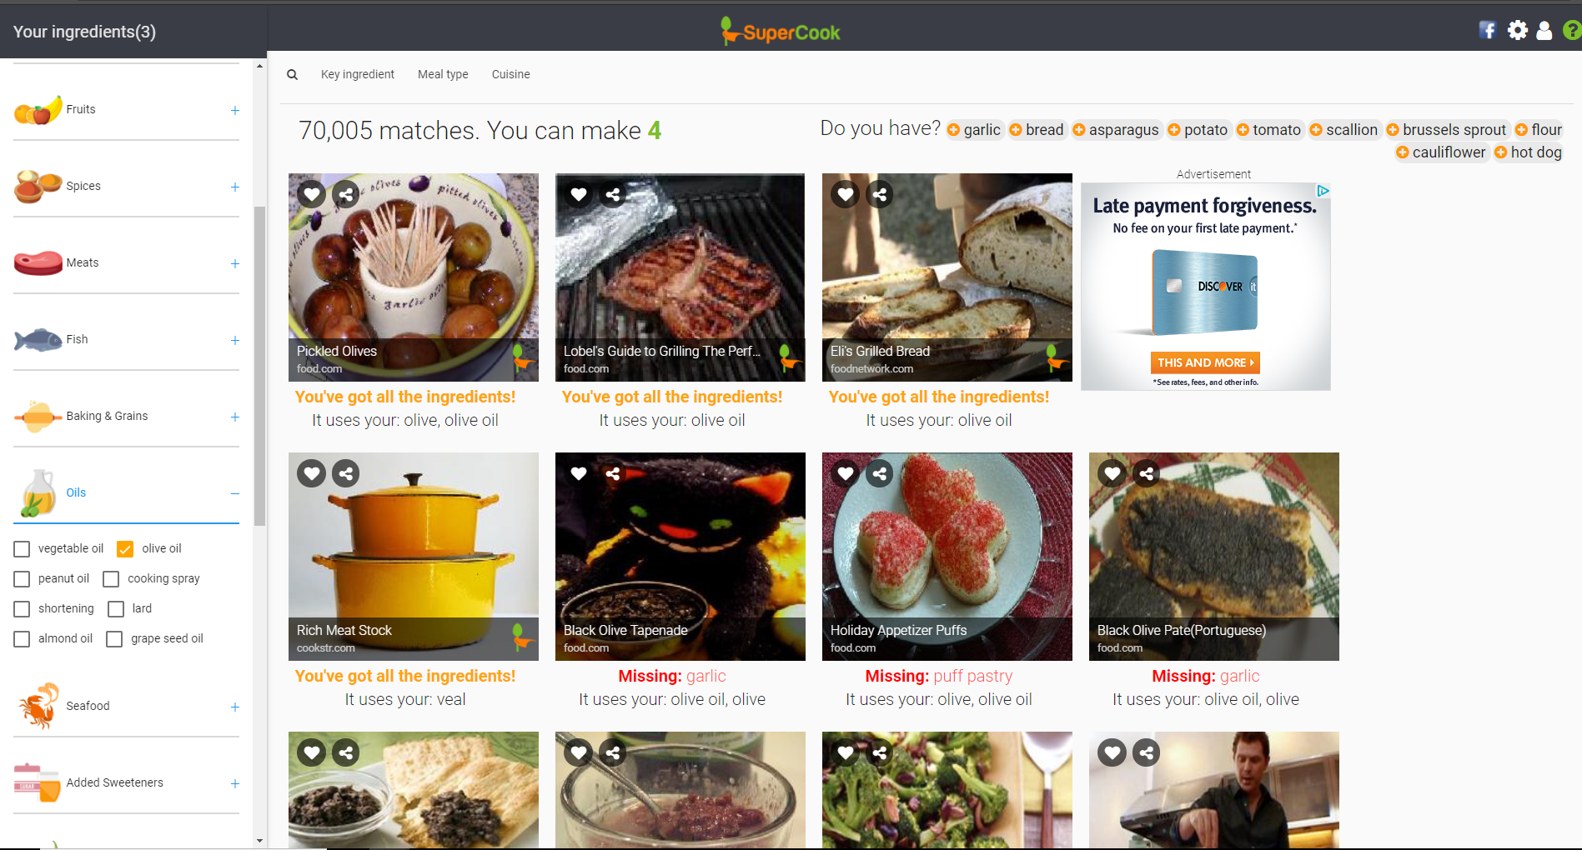
\includegraphics[width=0.8\columnwidth]{sc.png}\\
			\textbf{Figure \ref{fig:sc}:} SuperCook, a website, has standard features for a reverse cookbook, and has usability support such as compatibility with Alexa. However, it does not keep track of the amount of ingredient the user has or its expiration dates \cite{supercook}.
			\label{fig:sc}
		\end{figure}

	\subsubsection{\textbf{Cooking Fever Cookbook}; iOS app}
		\textit{Pros} - Easy and fluid cooking process walks the user through every step, allowing anyone to make any recipe as long as they have the equipment.\\
		\textit{Cons} - Does not include a pantry or ingredient lookup functionality.
		\begin{figure}[htb!]
		\centering
			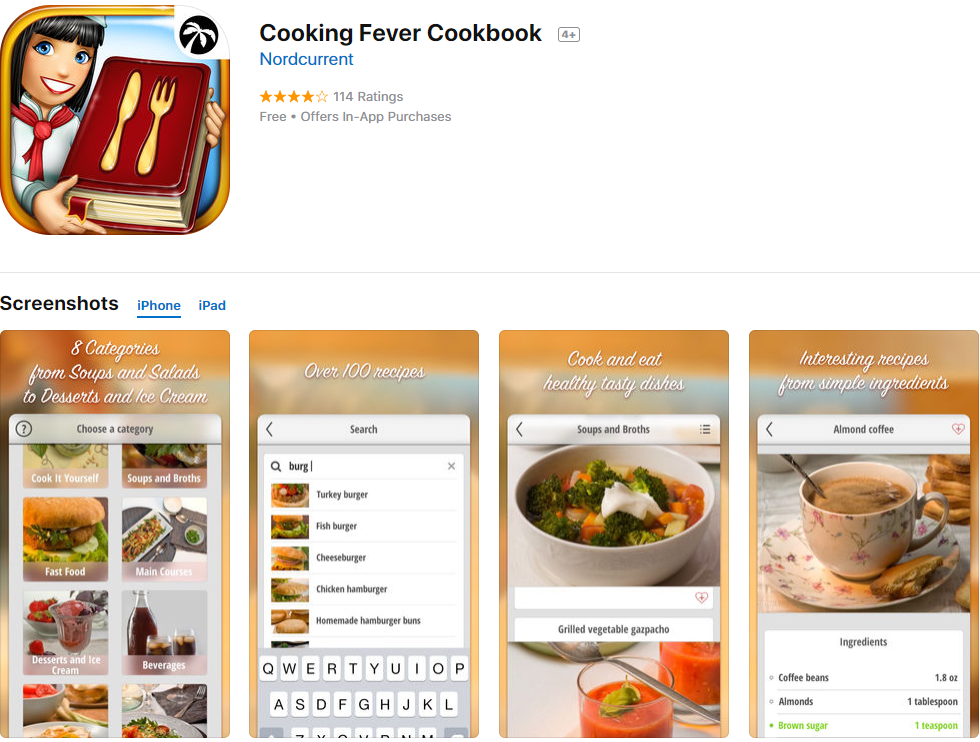
\includegraphics[width=0.8\columnwidth]{cfc.png}\\
			\textbf{Figure \ref{fig:cfc}:} Cooking Fever Cookbook, an iOS application, provides recipes that are easy to follow, but lacks on pantry management and ingredient search functionality \cite{cookingfever}.
			\label{fig:cfc}
		\end{figure}

	\subsubsection{\textbf{Handpick Recipes \& Ingredients}; Android and iOS app}
		\textit{Pros} - Text-based entry has autocomplete, which allows users to input of ingredients easily. Like SuperCook, this system also suggests additional ingredients to complete recipes, helping users discover new foods.\\
		\textit{Cons} - Text-based or dropdown entry is better than similar options but this is still clunkier than scanning. It does not accommodate quantity of items and does not factor in expiration dates.
		\begin{figure}[htb!]
		\centering
			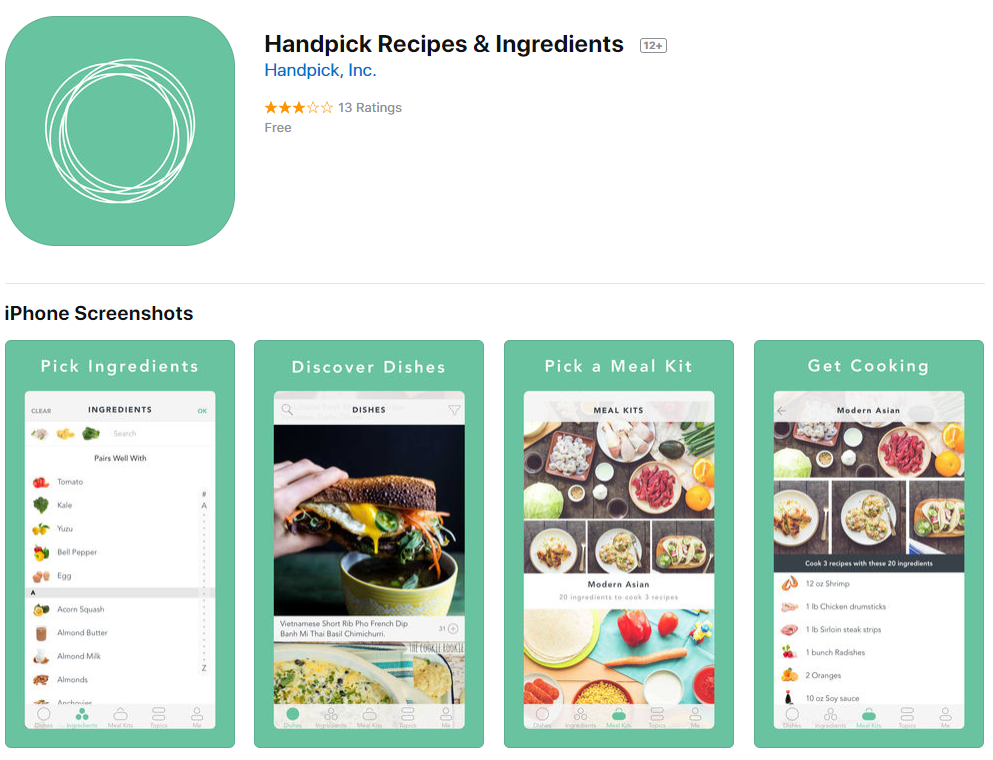
\includegraphics[width=0.8\columnwidth]{hpri.png}\\
			\textbf{Figure \ref{fig:hpri}:} Handpick Recipes \& Ingredients, a mobile application, while providing some useful functions such as ingredient recommendation, lacks others such as expiration checking and quantity tracking \cite{handpick}.
			\label{fig:hpri}
		\end{figure}

\subsection{Other Pantry Management Systems}\label{ssec:expirations}
	\subsubsection{\textbf{Pantry Check - Grocery List}; iOS app}
		\textit{Pros} - Easy ingredient entry via barcode scanning, which allows very rapid input of ingredients. Expiration date management also warns users when food is near expiration date.\\
		\textit{Cons} - Pantry Check does not include recipe functionality.
		\begin{figure}[htb!]
		\centering
			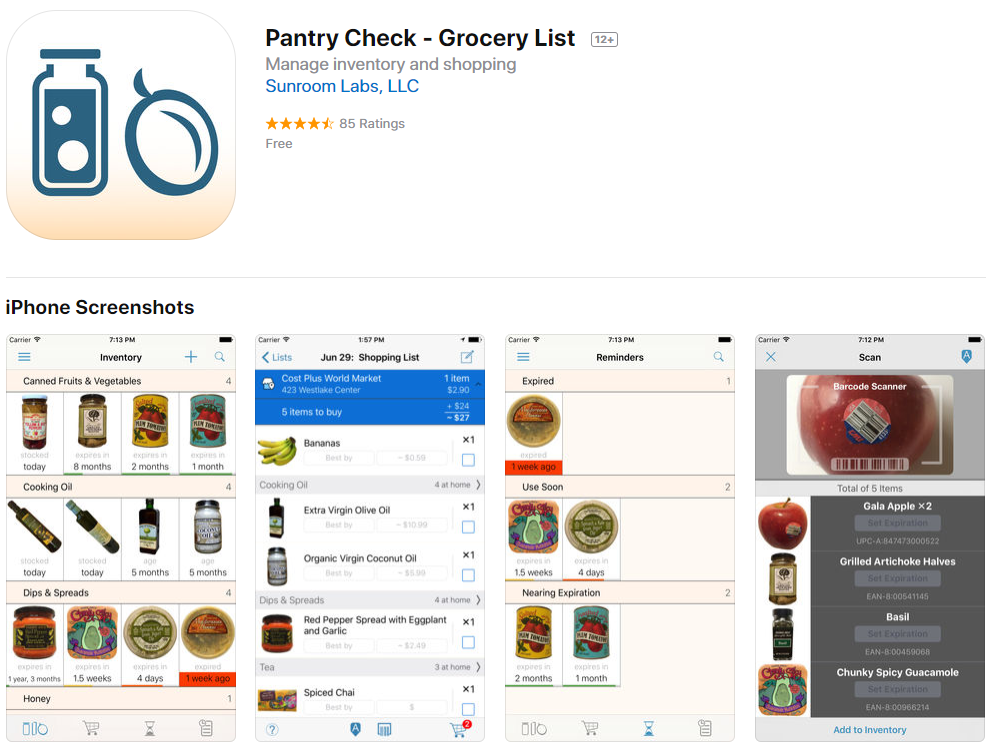
\includegraphics[width=0.8\columnwidth]{pantry_check.png}\\
			\textbf{Figure \ref{fig:pcheck}:} Pantry Check - Grocery List, an iOS application, shares some of the core ideas with Pantry Manager, but lacks recipe functionality \cite{pantrycheck}.
			\label{fig:pcheck}
		\end{figure}

	\subsubsection{\textbf{Samsung Family Hub 3.0 Refrigerator}; IOT}
		\textit{Pros} - Inventory management via internal cameras allow real-time view of food supply. Samsung Refrigerator allows users to order food via InstaCart or GrubHub and to share grocery lists for in-person shopping. \\
		\textit{Cons} - Costs over \$3000 for base model, with the most high-end model at around \$14000. It also does not include reverse-cookbook functionality or expiration date management
		\begin{figure}[htb!]
		\centering
			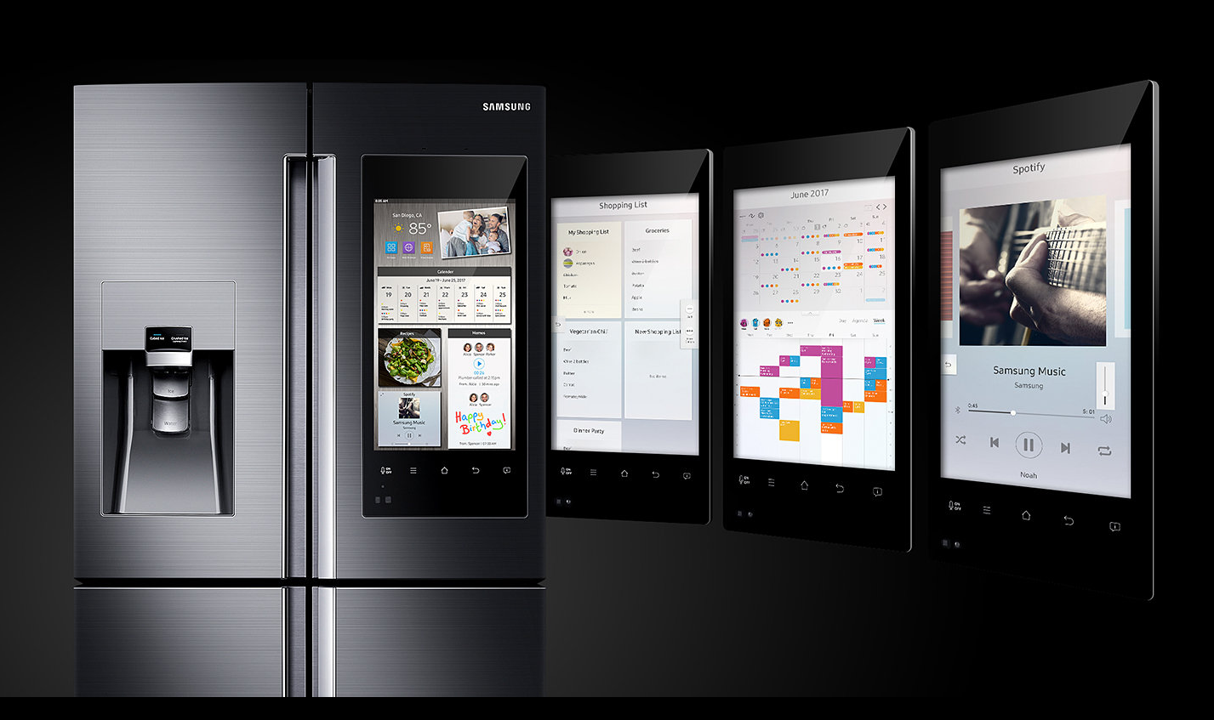
\includegraphics[width=0.8\columnwidth]{samsung_monster_fridge.png}\\
			\textbf{Figure \ref{fig:fridge}:} Samsung's Family Hub 3.0 fridge. While costly, the fridge provides a variety of useful functions such as internal camera for monitoring, inventory sharing, and ordering groceries. LG, one of Samsung's competitors in premium home appliances, also provides a similar line of smart fridges \cite{samsung}.
			\label{fig:fridge}
		\end{figure}

\subsection{Research}
	Most of the research pertaining to recipes revolves around algorithms to optimize recommendations. As part of our focus is providing tailored recommendations, this research is useful as a stretch goal. Ueda and colleagues suggest that while there is a large reservoir of websites and applications that allow users to find recipes, the recommendations are not tailored for the user's preference but rather on rating and filtering \cite{ueda}. Others including Yu lab suggest extensive use of filtering - including less directly related factors such as geography - to find better recommendations \cite{yu2011exploring}. Reversing the approach, as shown in Figure \ref{fig:deep}, Chen and Ngo suggest using deep learning to extract recipe and nutritious information given pictures of dishes \cite{chen2016deep}. Some focus on a more specialized field of substitute recommendations based on cooking actions \cite{shidochi2009finding}, while others suggest the method to sync multimedia presentations with text-based recipes for the users \cite{ide2010multimedia,doman2011video}. Such increase in scholarly studies about cooking and recipe recommendation may have been influenced by the recent trend in which college students, who tend to have large presence on the internet, are progressively relying on the web to discover recipes \cite{hertzler2002cooking}.
\begin{figure}[htb!]
	\centering
		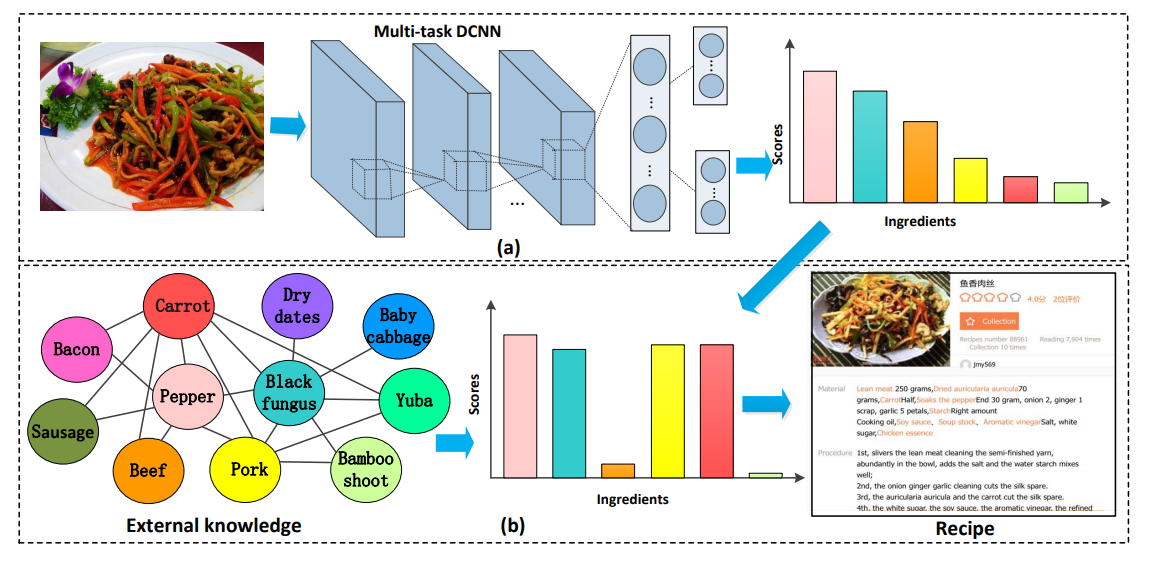
\includegraphics[width=0.8\columnwidth]{deep.png}\\
		\textbf{Figure \ref{fig:deep}:} Deep-based ingredient recognition system proposed by Chen and Ngo \cite{chen2016deep}. The user can use the neural net to recognize the ingredients in the dish, and in turn find the appropriate recipe that would result in the dish of interest.
		\label{fig:deep}
\end{figure}
    
% --------------- APPROACH --------------- %
\section{Approach}\label{Approach}
	\begin{figure}[htb!]
	\centering
		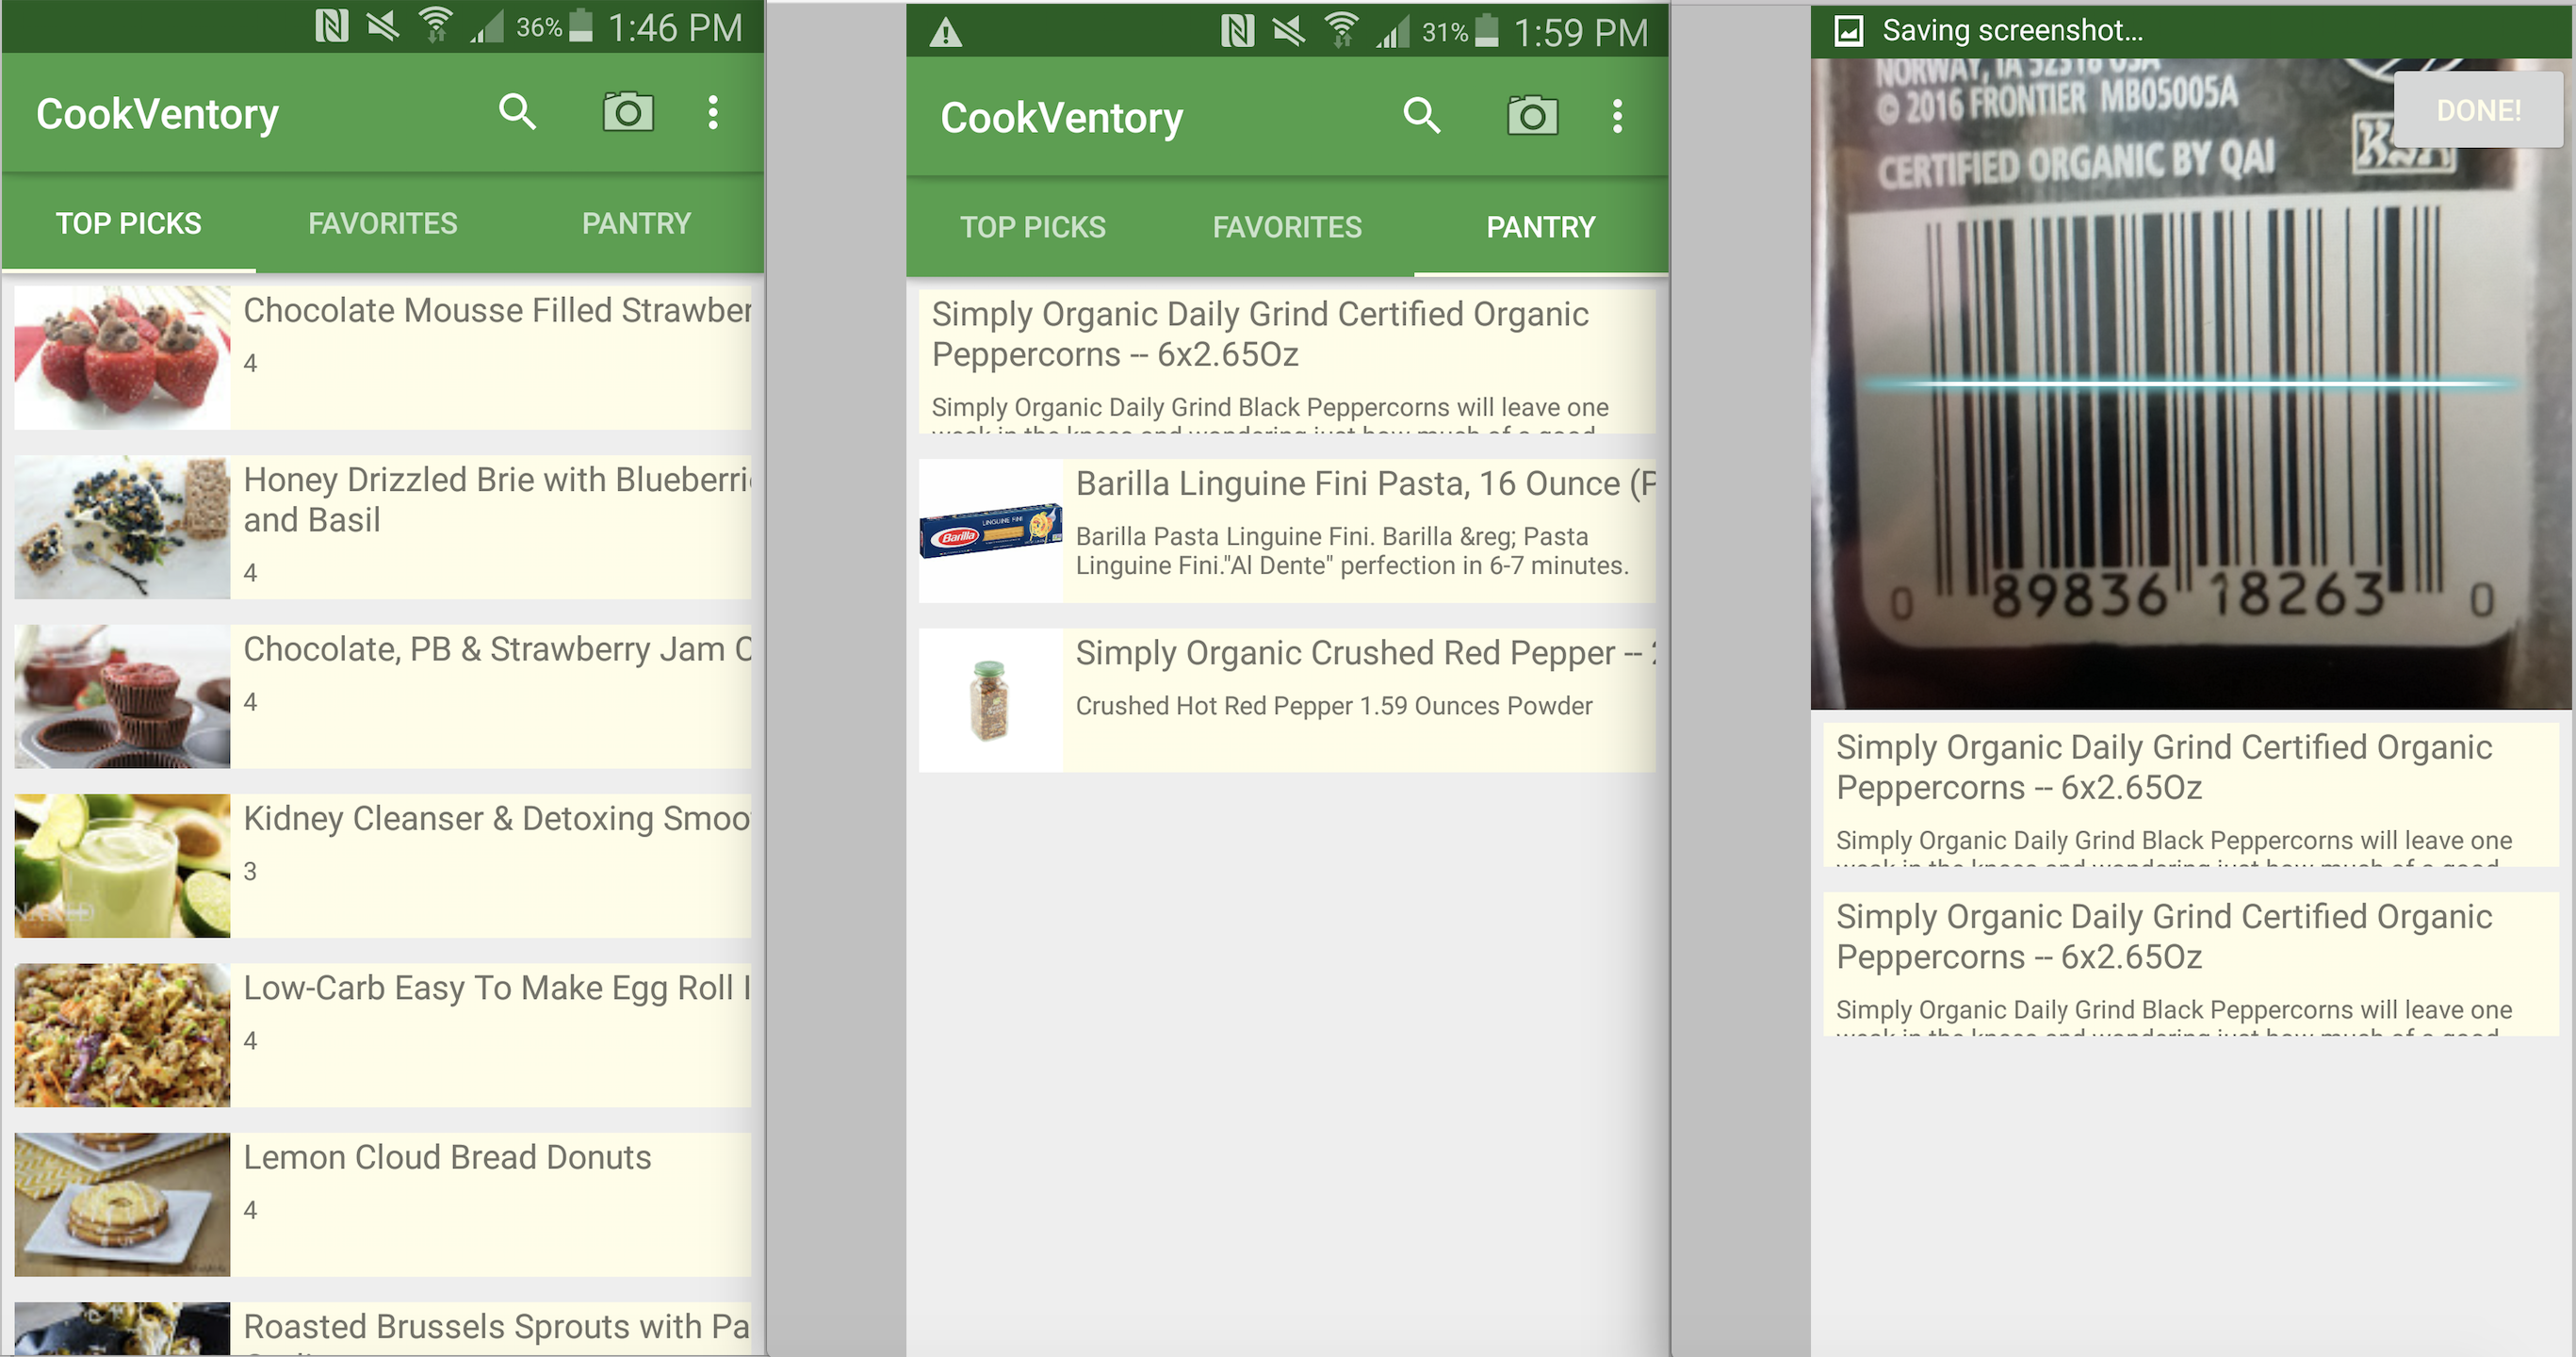
\includegraphics[width=0.8\columnwidth]{prototype.png}\\
		\textbf{Figure \ref{fig:prototype}:} CookVentory Prototype. The screenshots above show user interface during different stages of inputting ingredients.
		\label{fig:prototype}
	\end{figure}

	The goal of our user study was to assess user satisfaction with CookVentory as opposed to SuperCook, one of our major competitors. Specifically, we focused on assessing ingredient input method. CookVentory used barcode scanning approach while SuperCook utilized manually typed input. A working prototype of CookVentory used for this study focused mainly on necessary functionalities in order to perform ingredient inputting.

% --------------- METHODS --------------- %
\section{Methods}\label{methods}
\subsection{Participants}
	 The 37 test participants were informed of the purpose of the study before beginning. All individuals were provided snacks as compensation for participation (12-flavored gummy bears from Bowdoin C-Store and French Onion flavored Sun Chips). Four of the participants were further compensated with partial class credit. For the purpose of analysis, we excluded three of the participants from dataset as they failed to follow the experimental protocol.

\subsection{Materials}
\begin{itemize}
	\item The following ingredients were provided for each participants to enter into each of the provided programs.
	\begin{itemize}
		\item Barilla Linguine Fini
		\item Organic Black Peppercorns
		\item Mediterranean Sea Salt
		\item Simply Organic crushed red pepper
	\end{itemize}
	\item A Samsung Galaxy S5 (Android 5.0 SDK version 21) was provided with a prototype build of CookVentory and a bookmark of SuperCook's website.
	\item A set of sixteen (16) reaction words taken from the Microsoft Desirability Toolkit \cite{microsofttoolkit} were provided on a stack of index cards.
\end{itemize}
\begin{center}
\begin{tabular}{ |c|c| }
	\hline
		Positive Words & Negative Words \\ 
	\hline
		Responsive & Slow \\
		Intuitive & Confusing \\
		Satisfying & Stressful \\
		Consistent & Unpredictable \\
		Practical & Irrelevant \\
		Convenient & Inefficient \\
		Impressive & Busy \\
		Reliable & Distracting \\
 	\hline
\end{tabular}
\\~\\
\textbf{Table 1.} The set of reaction words that were provided to the participants to assess usability of both applications.
\end{center}

\subsection{Experiment Design}
\begin{itemize}
	\item Independent variable: Application used to input given ingredients, each using barcode scanning and manual input as the method of input.
	\item Dependent variable: User experience, as indicated by the \textit{top 4 words} from Microsoft Desirability Tool Kit.
	\item Control: As we performed repeated-measures design, we counterbalanced the order in which the tasks were performed; half of the participants tried CookVentory first whereas the other half started with SuperCook. We also randomized the order in which we presented our reaction words in a deck for each participant. \\
\end{itemize}
	 Our team provided our participants with a phone and a set of ingredients to input. Each participant was informed that their goal is to feed the system a set of ingredients and to retrieve recipes based on the input ingredients. They were also informed that the experiment focuses on the user experience of inputting ingredients by two methods: barcode scanning and manual text-based input.
	 The provided version of CookVentory opens to an initial interface that features recipe recommendations based on the ingredients saved in the pantry. Participants can scroll through the page to look at the list of recipes provided. They are also able to swipe left and right to view favorited recipes, a pantry of entered ingredients, and back to the new recipes page. (With our working prototype, participants were not able to click on a specific recipes listed on Top Picks or to add recipes to Favorites.) Upon clicking the camera button at upper right corner, the user is able to enter barcode scanning mode, which allows them to scan for UPC barcodes in order input ingredients to the pantry. Once scanned, an ingredient item is displayed underneath, which can be deleted or edited. Users can press the check button in order to save the ingredients scanned in the pantry or x button to exit out of barcode scanning. Participants can view the list of ingredients in the Pantry. \\~\\

\begin{figure}[htb!]
\centering
	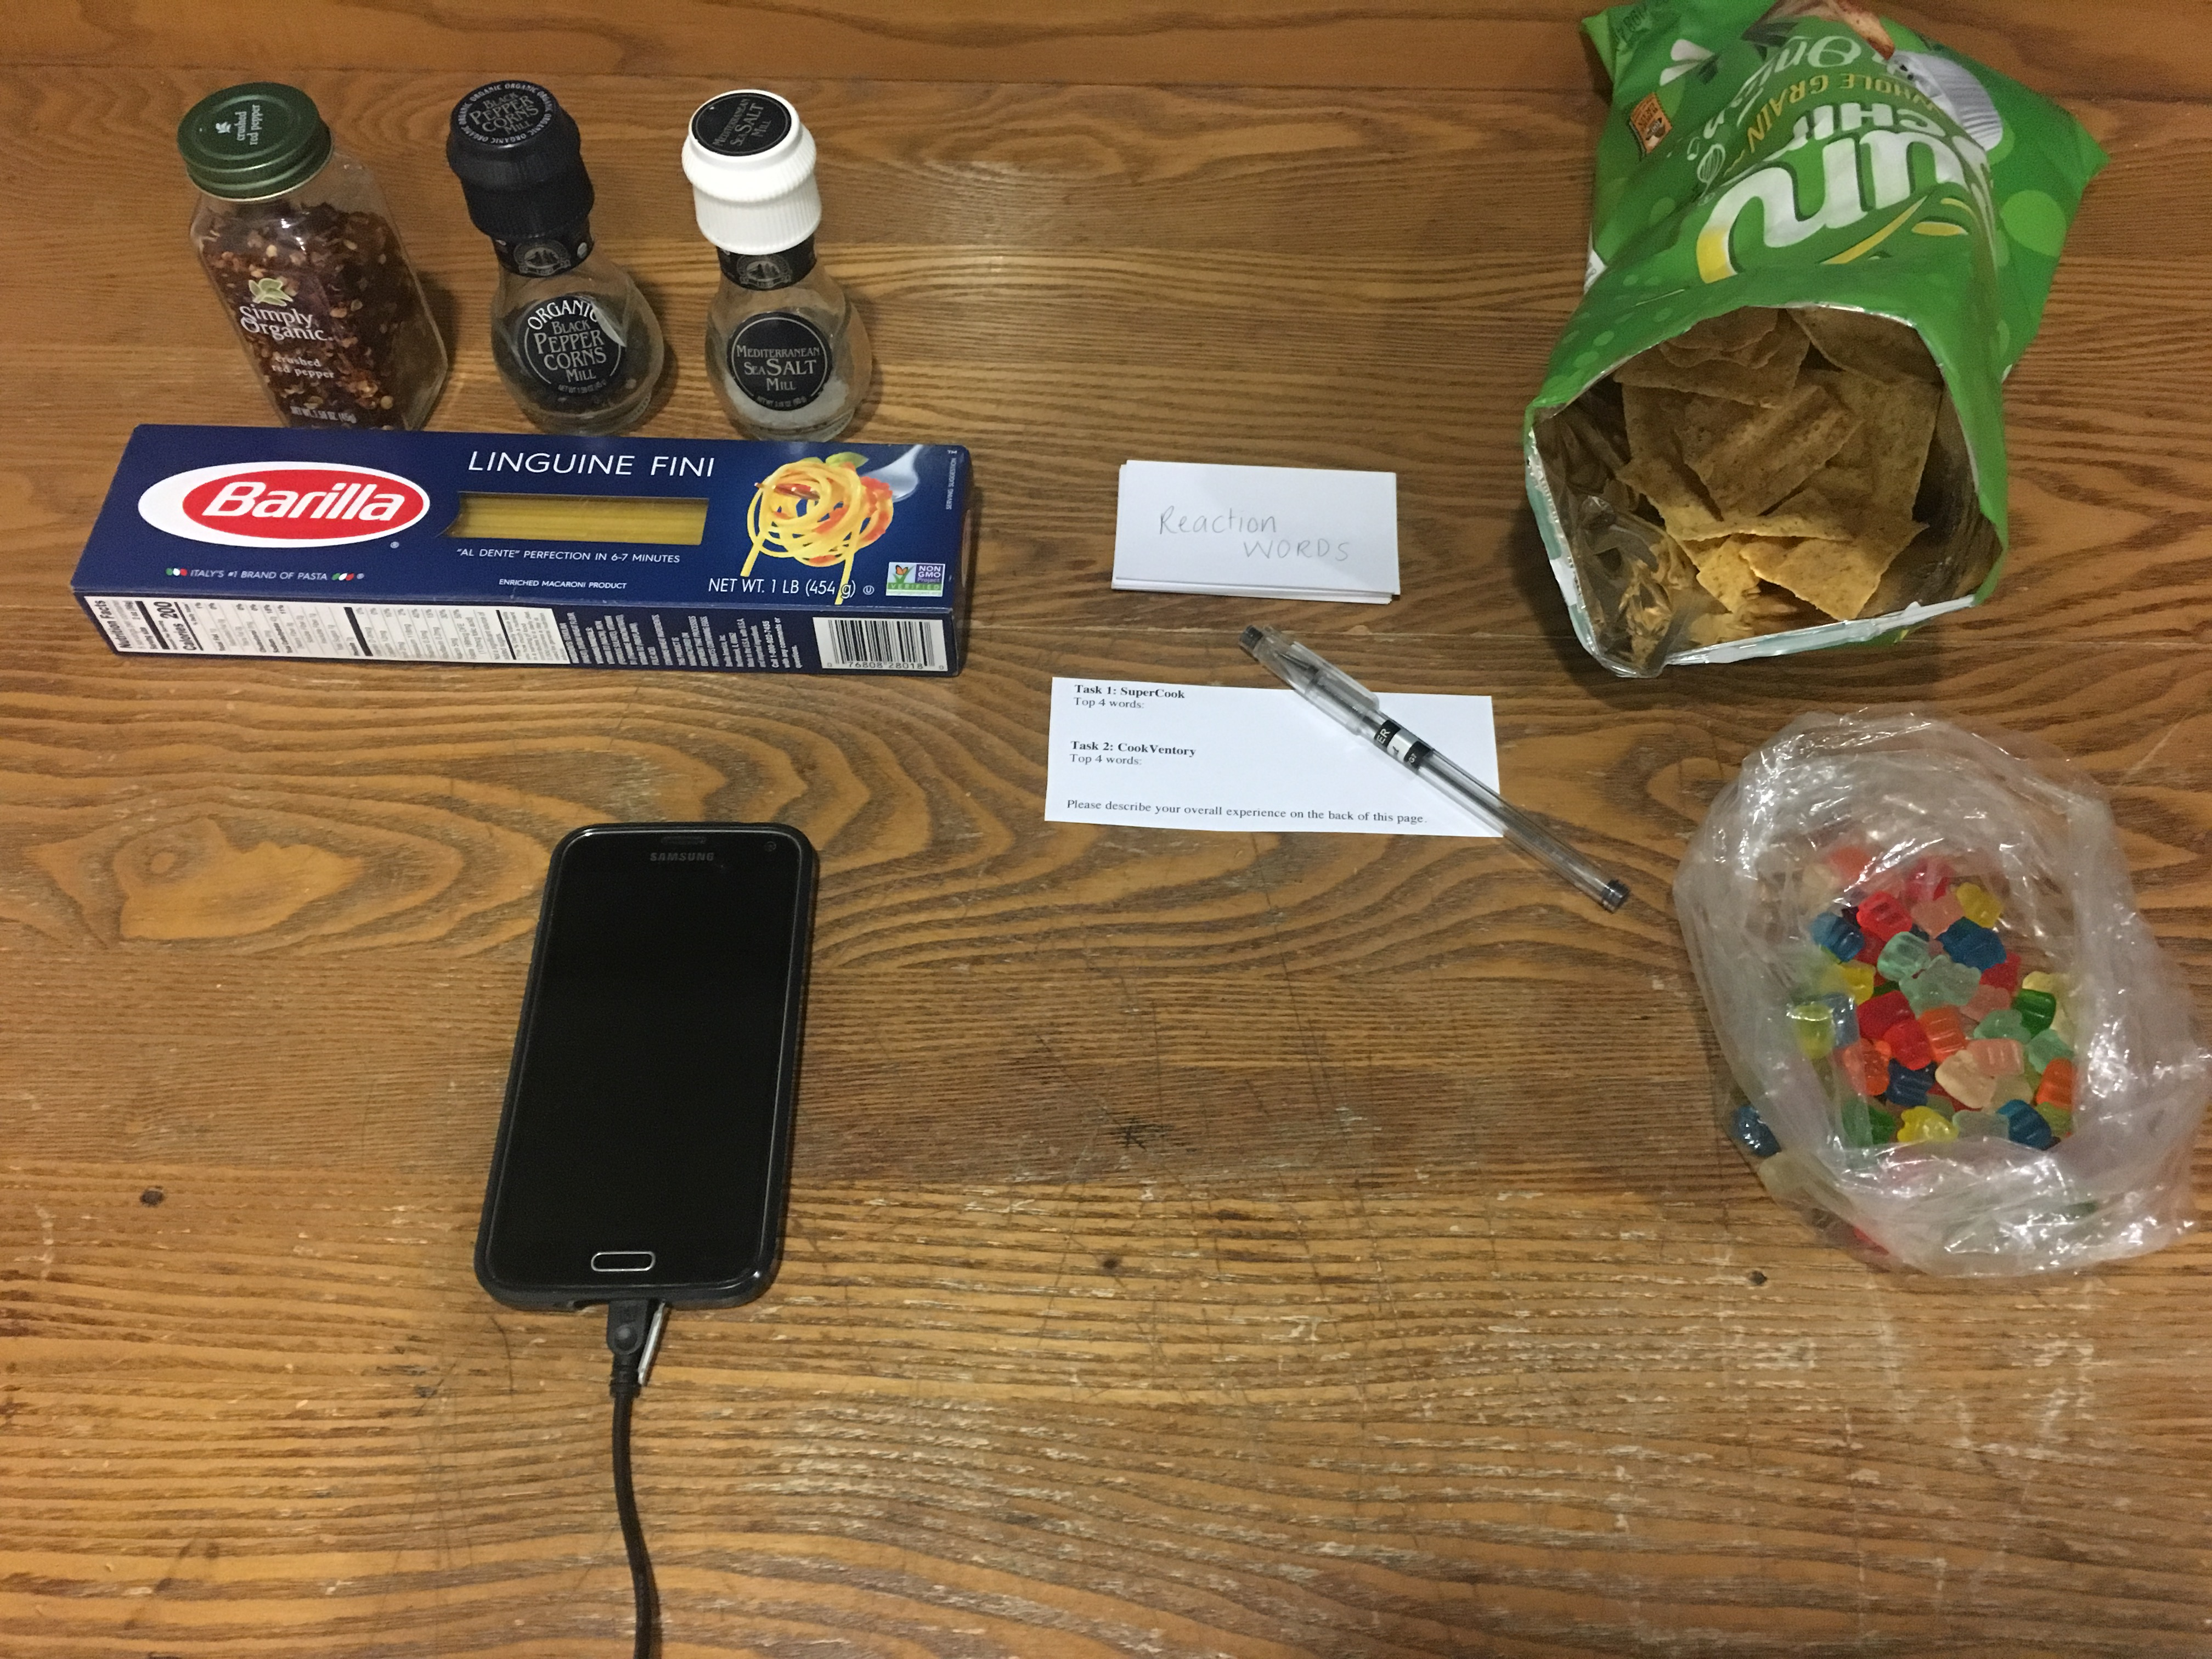
\includegraphics[width=0.8\columnwidth]{setup.jpg}\\
	\textbf{Figure \ref{fig:setup}:} The set up of the experiment. The ingredients, phone, appropriate questionnaire, and snacks were provided on the same platform. These were laid out before the participant in this exact formation.
	\label{fig:setup}
\end{figure}

\subsection{Procedure}
	 Each participant entered either Kanbar Control Room or Chamberlain Hall third floor study room to test CookVentory and SuperCook. On the table, we place one of two simple questionnaires (Figure \ref{fig:counterbalancing}) to record reaction words that would best describe their experience with both systems. On the back of the paper, we also asked each participant to provide feedback on their overall experience with both systems. Note that this study employed counterbalancing by alternating which portion of Figure \ref{fig:counterbalancing} was provided to each participant. Participants were not informed which application was ours.

\begin{figure}[htb!]
\centering
	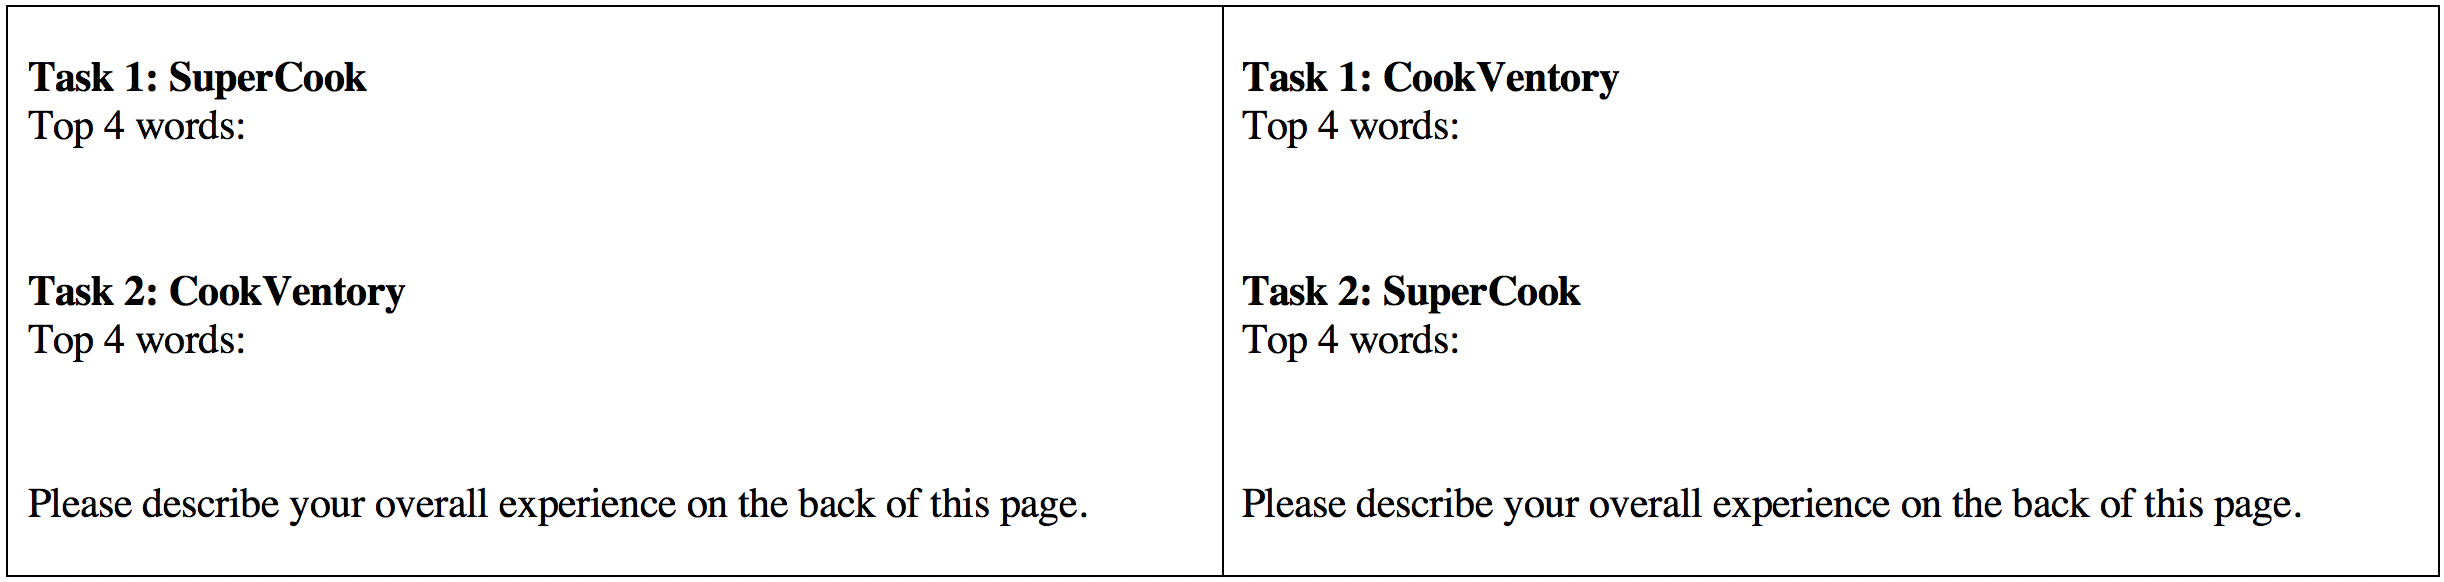
\includegraphics[width=0.8\columnwidth]{counterbalancing.png}\\
	\textbf{Figure \ref{fig:counterbalancing}:} Questionnaire. The form above was given to each participant to record reaction words for each system.
	\label{fig:counterbalancing}
\end{figure}

% --------------- RESULTS --------------- %
\section{Results}\label{results}
	Participants used more positive words to describe CookVentory (97 words) than SuperCook (53 words) -- 65\% of the total positive words recorded in the study were recorded for CookVentory. Among SuperCook-first participants, 64\% of all reported positive words were recorded to describe user experience with CookVentory. Similarly, 65\% of that among CookVentory-first participants were also for CookVentory. Our study also shows consistent results with reported negative words. Among SuperCook-first participants, 70\% of all negative words were used to describe SuperCook and 66\% of that were also recorded for our competitor among CookVentory-first participants. 

\begin{figure}[htb!]
\centering
	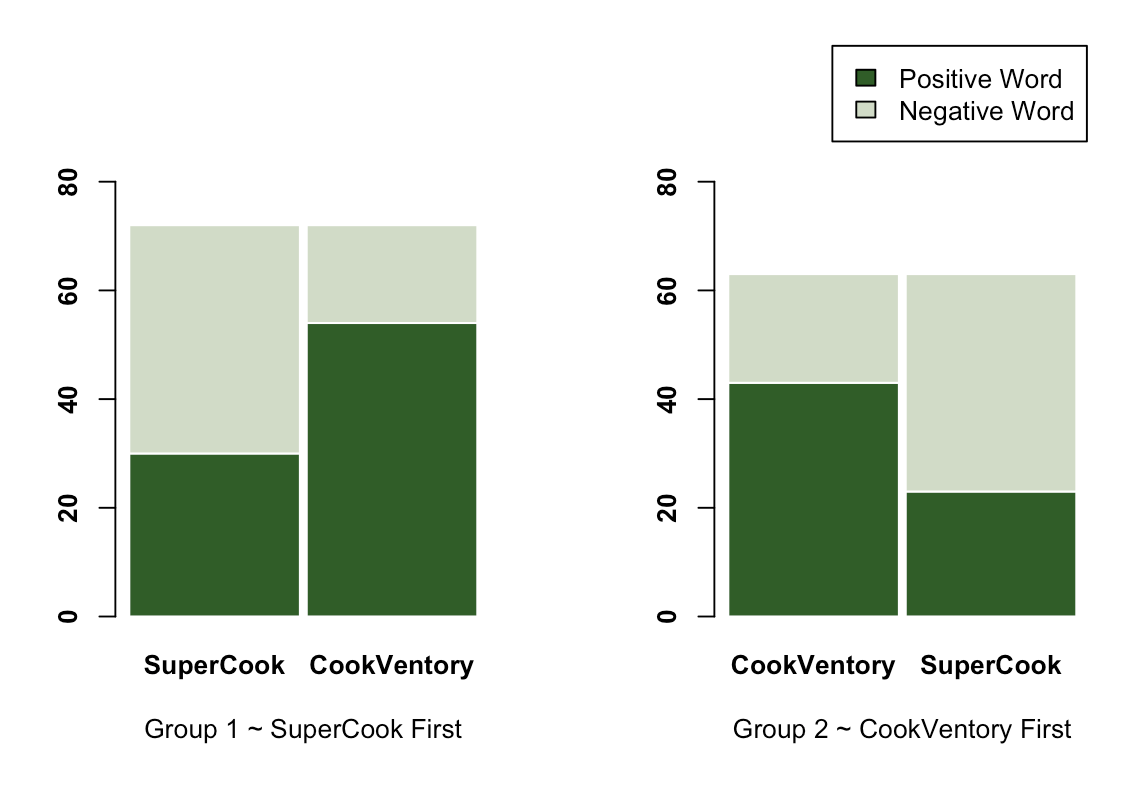
\includegraphics[width=0.8\columnwidth]{bar2.png}\\
	\textbf{Figure \ref{fig:bargraph}:} The raw frequency of positive and negative words reported by the participants.
	\label{fig:bargraph}
\end{figure}

\begin{center}
	\begin{tabular}{ |c|c|c| }
		\hline 
        	Positive Words & SuperCook & CookVentory \\ 
		\hline
			Responsive & 2 & 16\\
			Intuitive & 11 & 12\\
			Satisfying & 3 & 18\\
			Consistent & 3 & 4\\
			Practical & 18 & 13\\
			Convenient & 11 & 14 \\
			Impressive & 4& 12\\
			Reliable & 1 & 8\\
		\hline
	\end{tabular}
	\\~\\
	\textbf{Table 2.} Frequency of each positive reaction word for both interfaces. \\~\\
    
	\begin{tabular}{ |c|c|c| }
		\hline
			Negative Words & SuperCook & CookVentory \\ 
		\hline
			Slow & 19 & 4\\
			Confusing & 11 & 14\\
			Distracting & 5 & 0\\
			Stressful & 9 & 6\\
			Inefficient & 10 & 3\\
			Unpredictable & 15 & 7 \\
			Busy & 8& 2\\
			Irrelevant & 5 & 2\\
		\hline
	\end{tabular}
	\\~\\
	\textbf{Table 3.} Frequency of each negative reaction word for both interfaces.\\~\\~\\
\end{center} 

	Using McNemar's Test, we examined if one of SuperCook or CookVentory convinced participants to choose a specific reaction word to describe their user experience. 
    \begin{itemize}
	\item \textbf{Null Hypothesis:} Each reaction word is equally likely to be applied to either interface.
	\item \textbf{Alternative Hypothesis:} Either SuperCook or CookVentory convinced participants to choose the specified reaction word.
	\item \textbf{Let $\alpha$ = 0.05}. If p-value $< \alpha$, we reject the null hypothesis.
\end{itemize}

\begin{center}
	\begin{tabular}{|C|C|C|C|}
		\hline
			\textbf{Reaction Word} & \multicolumn{3}{ c |}{\textbf{CookVentory}} \\
		\cline{1-4} 
        	& \textbf{Test Result} & Yes & No \\
		\cline{2-4}
			\multirow{2}{*}{\textbf{SuperCook}} & Yes & A & B \\
		\cline{2-4}
			& No & C & D \\
		\hline
	\end{tabular}
	\\~\\
	\textbf{Table 4.} Contingency table setup. \\~\\~\\
\end{center}

In Table 4, A is the number of participants who reported the specified reaction to describe both interfaces. B is the number of participants who reported the specified reaction to describe SuperCook but not CookVentory. C is the inverse of B. D is the number of participants who did not report the specified reaction to either CookVentory or SuperCook. Note that A + B is the total number of participants who reported the specified reaction to describe SuperCook, and A + C is the total number reporting that reaction to CookVentory. The total sum of all the values in the table equals to 35, the total number of participants.





\begin{center}
	\begin{tabular}{|C|C|C|C|}
		\hline
			\textbf{Responsive} & \multicolumn{3}{ c |}{\textbf{CookVentory}} \\
		\cline{1-4}
			& \textbf{Test Result} & Yes & No \\
		\cline{2-4}
			\multirow{1}{*}{\textbf{SuperCook}} & Yes & 1 & 2 \\
		\cline{2-4}
			& No & 15 & 17 \\
		\cline{1-4}
			\multicolumn{4}{ | c |}{\textbf{McNemar's chi-squared = 8.4706, p-value = 0.003609}} \\
		\hline
	\end{tabular}
	\\~\\
	\textbf{Table 5.} Contingency table for \textit{Responsive}. \\~\\~\\
    
	\begin{tabular}{|C|C|C|C|}
		\hline
			\textbf{Satisfying}& \multicolumn{3}{ c |}{\textbf{CookVentory}} \\
		\cline{1-4}
			& \textbf{Test Result} & Yes & No \\
		\cline{2-4}
			\multirow{1}{*}{\textbf{SuperCook}}& Yes & 0 & 3 \\
		\cline{2-4}
			& No & 18 & 14 \\
		\cline{1-4}
			\multicolumn{4}{ | c |}{\textbf{McNemar's chi-squared = 9.3333, p-value = 0.00225}} \\
		\hline
	\end{tabular}
	\\~\\
	\textbf{Table 6.} Contingency table for \textit{Satisfying}.  \\~\\~\\
    
	\begin{tabular}{|C|C|C|C|}
		\hline
			\textbf{Reliable} & \multicolumn{3}{ c |}{\textbf{CookVentory}} \\
		\cline{1-4}
			& \textbf{Test Result} & Yes & No \\
		\cline{2-4}
			\multirow{1}{*}{\textbf{SuperCook}}& Yes & 0 & 1 \\
		\cline{2-4}
			& No & 8 & 26 \\
		\cline{1-4}
			\multicolumn{4}{ | c |}{\textbf{McNemar's chi-squared = 4, p-value = 0.0455}} \\
		\hline
	\end{tabular}
	\\~\\
	\textbf{Table 7.} Contingency table for \textit{Reliable}. \\~\\~\\
        
	\begin{tabular}{|C|C|C|C|}
		\hline
			\textbf{Inefficient}& \multicolumn{3}{ c |}{\textbf{CookVentory}} \\
		\cline{1-4}
			& \textbf{Test Result}& Yes & No \\
		\cline{2-4}
			\multirow{1}{*}{\textbf{SuperCook}}& Yes & 1 & 10 \\
		\cline{2-4}
			& No & 2 & 22 \\
		\cline{1-4}
			\multicolumn{4}{ | c |}{\textbf{McNemar's chi-squared = 4.0833, p-value = 0.04331}} \\
		\hline
	\end{tabular}
	\\~\\
	\textbf{Table 8.} Contingency table for \textit{Inefficient}.  \\~\\~\\
        
	\begin{tabular}{|C|C|C|C|}
		\hline
			\textbf{Slow}& \multicolumn{3}{ c |}{\textbf{CookVentory}} \\
		\cline{1-4}
			& \textbf{Test Result} & Yes & No \\
		\cline{2-4}
			\multirow{1}{*}{\textbf{SuperCook}}& Yes & 2 & 17 \\
		\cline{2-4}
			& No & 2 & 14 \\
		\cline{1-4}
			\multicolumn{4}{ | c |}{\textbf{McNemar's chi-squared = 10.316, p-value = 0.001319}} \\
		\hline
	\end{tabular}
	\\~\\
	\textbf{Table 9.} Contingency table for \textit{Slow}. \\~\\
\end{center} 

	It is important to note that the words in Tables 5 through 9 are the only ones that are significant. The words not reported above had p-values that are greater than $\alpha$, thus failing to reject our null hypothesis. These words are shown below:\\

\begin{center}
	\begin{tabular}{ |c|c|c|c| }
		\hline
			\textbf{Positive Word} & \textbf{p-value} & \textbf{Negative Word} & \textbf{p-value}\\ 
		\hline
			Intuitive &1& Confusing & 0.4533 \\
			Consistent & 0.7237 &Distracting & 0.07364 \\
			Practical & 0.332 & Stressful & 0.5791 \\
			Convenient & 0.4533 & Unpredictable & 0.06137 \\
			Impressive & 0.06137 & Busy & 0.1138 \\
			& & Irrelevant & 0.4497 \\
		\hline
	\end{tabular}
	\\~\\
	\textbf{Table 10.} Reaction words with p-value$ > \alpha$. ($alpha = 0.05$)\\~\\~\\
\end{center}

	 Based on our statistical analysis, one of the two interfaces provided convinced participants to pick the words \textit{Responsive}, \textit{Satisfying}, \textit{Reliable}, \textit{Inefficient}, and \textit{Slow}. We conclude that words \textit{Responsive} and \textit{Satisfying} were used to describe CookVentory. 46\% of participants used \textit{Responsive} for CookVentory while less than 1\% used the same word for SuperCook. Similarly, 51\% of participants used \textit{Satisfying} for CookVentory while less than 1\% used the same word for SuperCook.  On the other hand, most participants described SuperCook as \textit{Inefficient} and \textit{Slow}. For instance, 54\% of participants chose the word \textit{Slow} to describe SuperCook while 11\% of them to describe CookVentory. In Table 7, we concluded that \textit{Reliable} convinced participant to use for CookVentory. 23\% of participants used the word for our app while only 1 person used the same word for SuperCook. However, we also found that 70\% of all participants did not choose the word \textit{Reliable} to describe either CookVentory or SuperCook.\\~\\
     Among the words listed in Table 10, we found that there is an equal number of participants who recorded the word \textit{Intuitive} to describe both CookVentory and SuperCook. More participants also used \textit{Confusing} for CookVentory (43\%) than for SuperCook (31\%) \\. 
     

% --------------- DISCUSSION --------------- %
\section{Discussion}\label{discussion}
	We found that our participants were more likely to describe CookVentory with positive words than with negative words, confirming our hypothesis that barcode scanning would increase user satisfaction over text-based entry.
	As a result of our participant selection pool process, the vast majority of our test participants were Bowdoin College students. Further, many participants were personal friends of at least one of the researchers. This introduces a potential source of bias, as some of them may have been able to determine which of the two applications was ours and given it a more favorable review. Additionally, at least one researcher was present in the room for the experiments carried out in the Chamberlain Hall study room, which is a potential source of authority bias.
	Our findings confirm the KLM model of the interaction, which states that manual entry and scanning entry have identical descriptors with the exception of an additional homing step and typing for manual entry. Although we recorded higher user satisfaction with CookVentory, most participants did not describe the system as \textit{Reliable}, which could be another aspect of the app that we could test for future research. Interesting avenues for further research include evaluating the difference in error-aversity and speed between the two entry methods, and finding an even faster or more error-averse entry method, such as computer vision and recognition of ingredients. 

\balance{} % balance columns (to better equalize last page)
\bibliographystyle{SIGCHI-Reference-Format}
\bibliography{ref}

\end{document}
